% Chapter Template

\chapter{Hardware Testing and Results}\doublespacing % Main chapter title

\label{Chapter4} % Change X to a consecutive number; for referencing this chapter elsewhere, use \ref{ChapterX}

\lhead{Chapter IV. \emph{Hardware Testing and Results}} % Change X to a consecutive number; this is for the header on each page - perhaps a shortened title

%----------------------------------------------------------------------------------------
%	SECTION 1
%----------------------------------------------------------------------------------------






\section{Introduction}
% \noindent
We assess and define the performance of the accelerator by incorporating it into a System-on-Chip (SoC) that utilizes the AJIT Processor. This processor issues commands to the accelerator and retrieves the data. Additionally, the entire system is linked to a Network Interface Controller (NIC), which ensures high-speed input/output for rapid image loading into memory. The system's architecture is depicted in Figure 4.1.
\begin{figure}[h]
    \centering
    % \includegraphics[width=\linewidth]{Chapters/Chapter_4/images/vcu128.jpg}
    \includegraphics[width=\linewidth]{../figures/vcu128.jpg}
    \caption{Block Diagram for SoC}
    % \label{fig:your_label}
\end{figure}
\\
The system features a 32-bit wide AJIT processor at its core. This processor uses an ACB interface to interact with memory and other modules. The AFB interface, connected to the Network Interface Controller (NIC) and the accelerator engine, is utilized to transfer configuration data from the processor and relay status flags back to it. The modules also have an ACB interface for memory access. The memory subsystem includes a DRAM controller linked to an ACB to UI conversion protocol, which translates memory requests from the ACB bus to DRAM requests and vice versa for responses. Additionally, the processor is equipped with a couple of UART interfaces for external communication. The NIC also has an interface to connect with the Xilinx MAC IP, enabling communication with the host machine via Ethernet, currently configured to operate at 100Mbps.

% This chapter provides an overview of the initial survey, which encompasses survey site selection, data collection with the help of videography, pedestrian selection, and the extraction and coding of variables from the collected data.



\subsection{Processor Code}
% \lipsum[2]
Below algorithm details the functioning of the processor code. It begins by initializing the memory spaces required by all modules, including the NIC queues, the kernel addresses for the accelerators, and the memory spaces for receiving and storing tensors during engine computation. Once the memory spaces are initialized, all NIC queues are configured and initialized, and the Network Interface Controller starts operating. The kernels are then fetched via Ethernet, followed by the input tensors . With the setup complete, the NIC is turned off, and the engine process the data stage by stage. After processing all the stages, the output data is sent to the host PC via Ethernet, where the results are verified for accuracy.
\begin{algorithm}
\caption{Pseudocode for processor}
\begin{algorithmic}[1]
    \STATE Initialize memory spaces for all modules:
    \STATE \quad \textbullet\ NIC queues
    \STATE \quad \textbullet\ Kernel addresses for accelerator
    \STATE \quad \textbullet\ Memory spaces for receiving and storing tensors
    \STATE Configure and initialize all NIC queues
    \STATE Start Network Interface Controller
    \STATE Fetch kernels via Ethernet
    \STATE while 1 do
    \STATE \quad Fetch input tensor via Ethernet
    % \STATE Turn off NIC
    \STATE \quad  Process the input
    \STATE \quad Send output data to host PC via Ethernet
    \STATE end while
\end{algorithmic}
\end{algorithm}

\section{NIC Interface}
The processor initializes the NIC queues and activates the NIC. Upon receiving data from the MAC, the NIC retrieves an address from the free queue, which contains addresses of empty packet buffers, and writes the packet to that buffer. After successfully writing the packet, the NIC places the buffer's address into the RX queue. An address in the RX queue signifies that a packet has been received and requires processor action. During this process, the processor continuously polls the RX queue. Upon detecting data, it reads the packet and makes a decision. The processor then stores the packet in a shared memory location accessible to the accelerator through its registers. Once the packet storage is complete, the processor places the address into the TX queue, serving as an acknowledgment for the host. Upon receiving this acknowledgment, the host sends a new packet. This describes the overall process for storing files in memory.\\
To transmit a file via the Ethernet interface, the processor first breaks the file into multiple packets. It then retrieves an empty buffer address from the free queue and stores each packet at the corresponding address. Once the packet is successfully stored, the processor pushes the buffer address into the TX queue. The NIC's transmit engine, which continuously polls the TX queue, reads the buffer and sends the packet out. This process is repeated until all packets are transmitted.

\section{Accelerator Interface}
% \lipsum[1]
The processor begins by loading data into registers 1 to 12. It then sets bits 0 and 2 of register 0, signaling the accelerator to commence operation. The processor can either proceed with other tasks or poll register 0, awaiting the completion signal indicated by bit 3 of register 0 being set high. Once the accelerator completes its task, the processor updates the registers with the parameters for the next stage or image.\\
Additionally, the accelerator is managed by a control daemon that resets the registers, reads data from the AFB ACCELERATOR REQUEST, writes this data to the accelerator registers, and sends back a response to the AFB ACCELERATOR RESPONSE. This control daemon runs continuously, waiting for requests from the processor on the AFB ACCELERATOR REQUEST.\\
The accelerator also includes a worker daemon that monitors the r0 register for specific bits to be set. When the processor issues an execution request through the registers, the worker daemon invokes the core function with the parameters stored by the processor in other registers. Upon completing the execution, it sets bit 3 of r0 back to 0, signaling to the processor that the computation is finished.\\


\newpage

\section{Results}
% \lipsum[1-2]
\begin{table}[h]
    \centering
    \begin{tabularx}{1.1\textwidth}{|c|X|X|c|}
        \hline
        \textbf{Sr.No} & \textbf{Platform}  & \textbf{Datatype for storage} & \textbf{Accuracy} \\
        \hline
        1 &  CPU & 32 bit float    & 98.27\% \\
        \hline
        2 &  CPU & UINT8    & 98\% \\
        \hline
        3 &  FPGA & UINT8    & 98\% \\
        \hline


    \end{tabularx}
    \caption{Comparison of LeNet Architecture on Different Platforms}
    \label{tab:lenet_comparison}
\end{table}


% \subsection{Data Extraction and Coding}
% \lipsum[13]



% \section{Summary}
% \lipsum[4]






%%%%%%%%%%%%%%%%% Changes%%%%%%%%%%%%%%%%%%%%%%%%














































